\begin{pa} \label{PA:10.6} Wind Chill $f$ (in degrees Fahrenheit) is the term used to describe how cold it feels based on the actual temperature $x$ (in degrees Fahrenheit) and the wind speed $y$ (in miles per hour). For example, if it is 10 degrees and the wind is blowing at 5 miles per hour, then it feels as though the temperature is about 1.2 degrees Fahrenheit. A formula\footnote{\url{http://www.crh.noaa.gov/ddc/?n=windchill}} for wind chill is given by
\[f(x, y) = 35.74+0.6215x-35.75y^{0.16}+0.4275xy^{0.16}.\]
Suppose we want to determine how the wind chill changes at the point (10,5) if the wind speed and temperature each increase in a 3:1 proportion.  (in other words, in the direction of the vector $\vv = \langle 3,1 \rangle$).
    \ba
    \item Find a unit vector $\vu = \langle u_1, u_2 \rangle$ in the direction of $\vv$.



\begin{comment}

We find a unit vector in the direction of $\vv$ by dividing $\vv$ by its magnitude. So
\[\vu = \left(\frac{1}{\sqrt{10}}\right) \langle 3,1 \rangle.\]



\end{comment}


\begin{figure}[h]
\begin{center}
\resizebox{!}{2.0in}{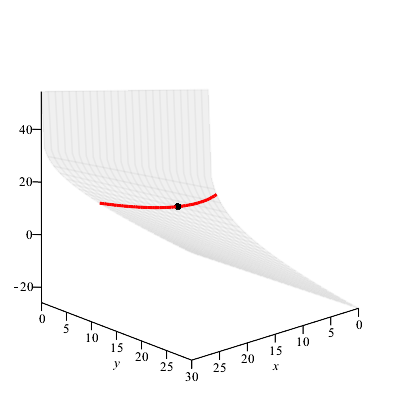
\includegraphics[trim=0cm 0cm 1cm 2cm, clip]{10_6_Wind_chill_surface}}
\end{center}
\caption{The wind chill surface.}
\label{F:10.6.Wind_chill}
\end{figure}
%crop graphics in animate trim=<left> <bottom> <right> <top>, add, clip with \includegraphics

    \item The direction of the unit vector $\vu$ defines a curve on the surface from the point $(10,5)$ as shown in Figure \ref{F:10.6.Wind_chill}. To stay on this curve from the point $(10,5)$, if $x$ changes by an amount $u_1$, then $y$ must change by an amount $u_2$. Use this idea to find a parameterization $\langle x(t), x(t) \rangle$ of the line in the plane through the point $(10,5)$ in the direction of the vector $\vu$. Set up your parameterization so that $x(0) = 10$ and $y(0) = 5$.

\begin{comment}

A parameterization $\langle x(t), y(t) \rangle$ of the line in the plane through the point $(10,5)$ in the direction of the vector $\vu$ is
\[x(t) = 10 + u_1t, \ \ \ \ y(t) = 5+u_2t.\]



\end{comment}

    \item The parameterization of the line in part (a) provides a way to write $f$ as a function of $t$ and describe the $z$ coordinates of the points on the curve on the surface defined by the vector $\vu$, as shown in Figure \ref{F:10.6.Wind_chill}. So along this curve we can consider $f$ as a function of $t$. Use the Chain rule to show that
        \begin{equation} \label{eq:10.6.DD_formula}
        \frac{df}{dt}\biggm|_{t=0} = f_x(10,5) u_1 + f_y(10,5) u_2.
        \end{equation}
        (Hint: How are $\ds \frac{dx}{dt}\biggm|_{(10,5)}$ and $\ds \frac{dy}{dt}\biggm|_{(10,5)}$ related to $u_1$ and $u_2$?)



\begin{comment}

The Chain Rule states that
\[\frac{df}{dt} = \frac{\partial f}{\partial x} \frac{dx}{dt} + \frac{\partial f}{\partial y} \frac{dy}{dt}.\]
At the point $(10,5)$ (when $t=0$) and along the curve on the surface determined by the vector $\vu$, we have ${\ds \frac{dx}{dt}\biggm|_{t=0} = u_1}$ and ${\ds \frac{df}{dt}\biggm|_{t=0} = u_2}$. So
\[\frac{df}{dt}\biggm|_{t=0} &= f_x(10,5) u_1 + f_y(10,5) u_2.\]



\end{comment}

    \item Use the result from part (c) to approximate the value of $\ds \frac{df}{dt}\biggm|_{t=0}$ to three decimal places. Interpret the result in the context of wind chill.



\begin{comment}
%\[f(x, y) = 35.74+0.6215x-35.75y^{0.16}+0.4275xy^{0.16}.\]
In this case we have
\[f_x(x,y) =  0.6215+0.4275y^{0.16} \ \ \ \ \text{ and } \ \ \ \ f_y(x,y) = (5.72+0.0684x)y^{-0.84}.\]
So
\begin{align*}
\frac{df}{dt}\biggm|_{t=0} &= f_x(10,5) \left(\frac{3}{\sqrt{10}}\right) + f_y(10,5) \left(\frac{1}{\sqrt{10}}\right) \\
    &approx (1.175) \left(\frac{3}{\sqrt{10}}\right) + (-1.303) \left(\frac{1}{\sqrt{10}}\right)  \\
    &\approx 0.993.
\end{align*}
This number tells us that if we increase the temperature and wind speed at the point $(10,5)$ in the ratio of 3:1, then wind chill will increase by approximately 1 degree Fahrenheit.



\end{comment}


    \ea

\end{pa} \afterpa 